\documentclass{gmto}


\usepackage{amsmath}
\usepackage[load=accepted]{siunitx}
\usepackage{todonotes}
\usepackage{booktabs}
\usepackage{amsfonts}

\DocID{GMT-XXX-\#\#\#\#}
\DocVersion{1.0}
\DocStatus{Draft}

\addbibresource{gmt.bib}

\title{GMT Integrated Model with ASMS}
%\subtitle{}
\author{R. Conan, R. Romano, C. Dribusch, P. Thompson}
\date{\today}

\begin{document}

\maketitle

\clearpage

\section*{Signatures}
\vspace{1cm}
\subsection*{Author}
\vspace{1.5cm}
%\tabulinesep=1em
\begin{tabu} to \linewidth {X[3,l]X[1,l]}
  \rule{\linewidth}{.1pt} & \rule{\linewidth}{.1pt} \\
  Name, title & Date
\end{tabu}
\vspace{1.5cm}
\subsection*{Approvers}
\vspace{1.5cm}
%\tabulinesep=1em
\begin{tabu} to \linewidth {X[3,l]X[1,l]}
  \rule{\linewidth}{.1pt} & \rule{\linewidth}{.1pt} \\
  Name, title & Date \\[1cm]
  \rule{\linewidth}{.1pt} & \rule{\linewidth}{.1pt} \\
  Name, title & Date
\end{tabu}

\clearpage

\section*{Revision Log}

\begin{revisions}
  1.0 & \today & All & None & Initial version & Author \\  
\end{revisions}

\clearpage

\tableofcontents
\listoffigures
\listoftables

\clearpage

\section{Purpose}
\label{sec:purpose}

The document describes the GMT integrated model in its version with the ASMS FEM
and ASMS inner control system.

\section{Introduction}
\label{sec:introduction}

\section{Integrated model}

\subsection{Integrated model}
\label{sec:im}

\subsection{FEM}
\label{sec:fem}


% \begin{itemize}
% \item FEM description e.g. ODC mount FEM, M1 FEM, frequency range, ...
% \item pretty pictures of the whole FEM and the top-end + ASMS part
% \item ...
% \end{itemize}

The finite element mesh of the telescope is the basis of a linear state space model that utilizes modal and static solutions of the FEM. Modes are obtained from 0 to 1475 Hz. 
To reduce the number of modes to a manageable number a constraint is added when solving for modes above 75 Hz The constraint fixes all nodes below the truss interface of the topend. 
The static solution is employed to correct the DC gain of the state space model which is due to omitting higher frequency modes as well as the additional constraint.

ASM cells and corresponding cabinets are attached to the top-end frame. 
The ASM is current as of June 2021.
The ASM mesh features flexible facesheets held in place by flexures around its rim. 
To actuate the facesheet and to simulate wind disturbance forces and moments may be applied which are spread via an interpolation element (RBE3). 
In the case of actuation equal and opposite reactions are applied to the cold plate. Similarly forces may be applied between the reference body and the facesheet to simulate fluid damping. The voice coil actuators are not explicitly modeled to avoid a large number of extra modes. 
The ASM cells may be positioned by changing the lengths of the positioners via axial forces.

The mount is current as of April 2021, and the configuration is 0 deg azimuth and 30 deg zenith. 
The mount is ``unlocked'', such that the  azimuth, elevation and GIR rotation angles can be controlled via feedback controllers utilizing drives and encoders.
 
M1 segments are explicitly modeled in detail, including honeycomb and load spreaders. 
M1 pneumatic actuators are implemented as forces applied to load spreaders on the back surface of the M1 segments with reaction forces applied to the top-plate of the M1 segments. 
The M1 segments may be positioned by changing the length of the hardpoints (rod elements) via axial forces.

The pier mesh is the mesh used by the mount vendor as of June 2021. It is not the model currently generated by IDOM.

It would be easy to have errors in the setup of the FE model, for example forces applied to the wrong node. 
To reduce the likelihood of such errors extensive (but not exhaustive) tests validate the inputs and outputs of the model. 
For example one automated check tests that the mirror segments move as expected for given inputs to the hardpoints and positioners.
The current test suite covers the positioning of M1 and M2 segments, mount
drives and encoders as well as some more general stiffness tests, but not the
active optics on M1 and M2.

\begin{figure}
  \centering
  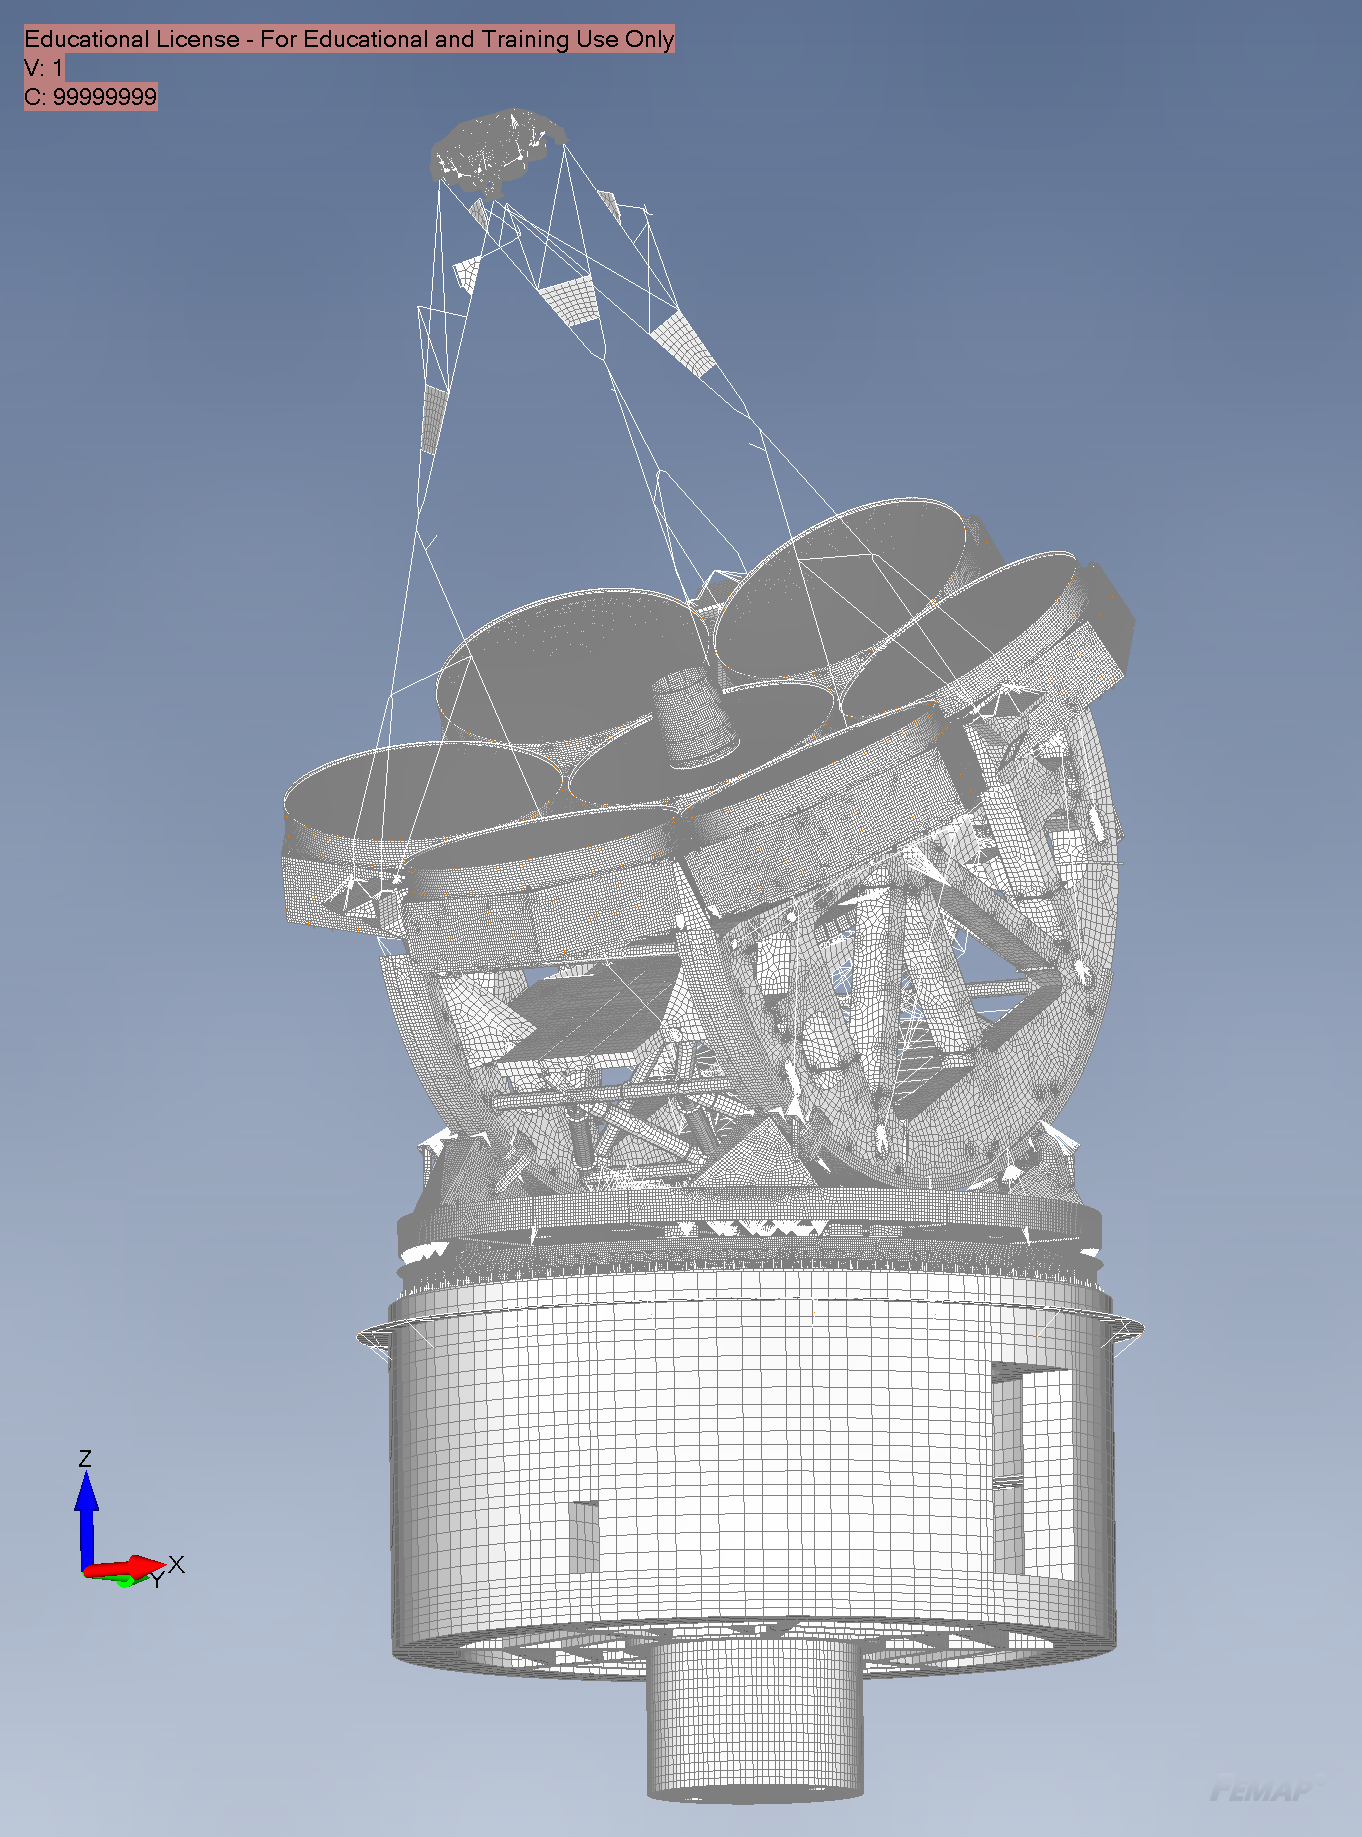
\includegraphics[width=0.5\textwidth]{FEM/whole_telescope.png}
  \caption{Whole telescope FEM.}
  \label{fig:fem-whole}
\end{figure}

\begin{figure}
  \centering
  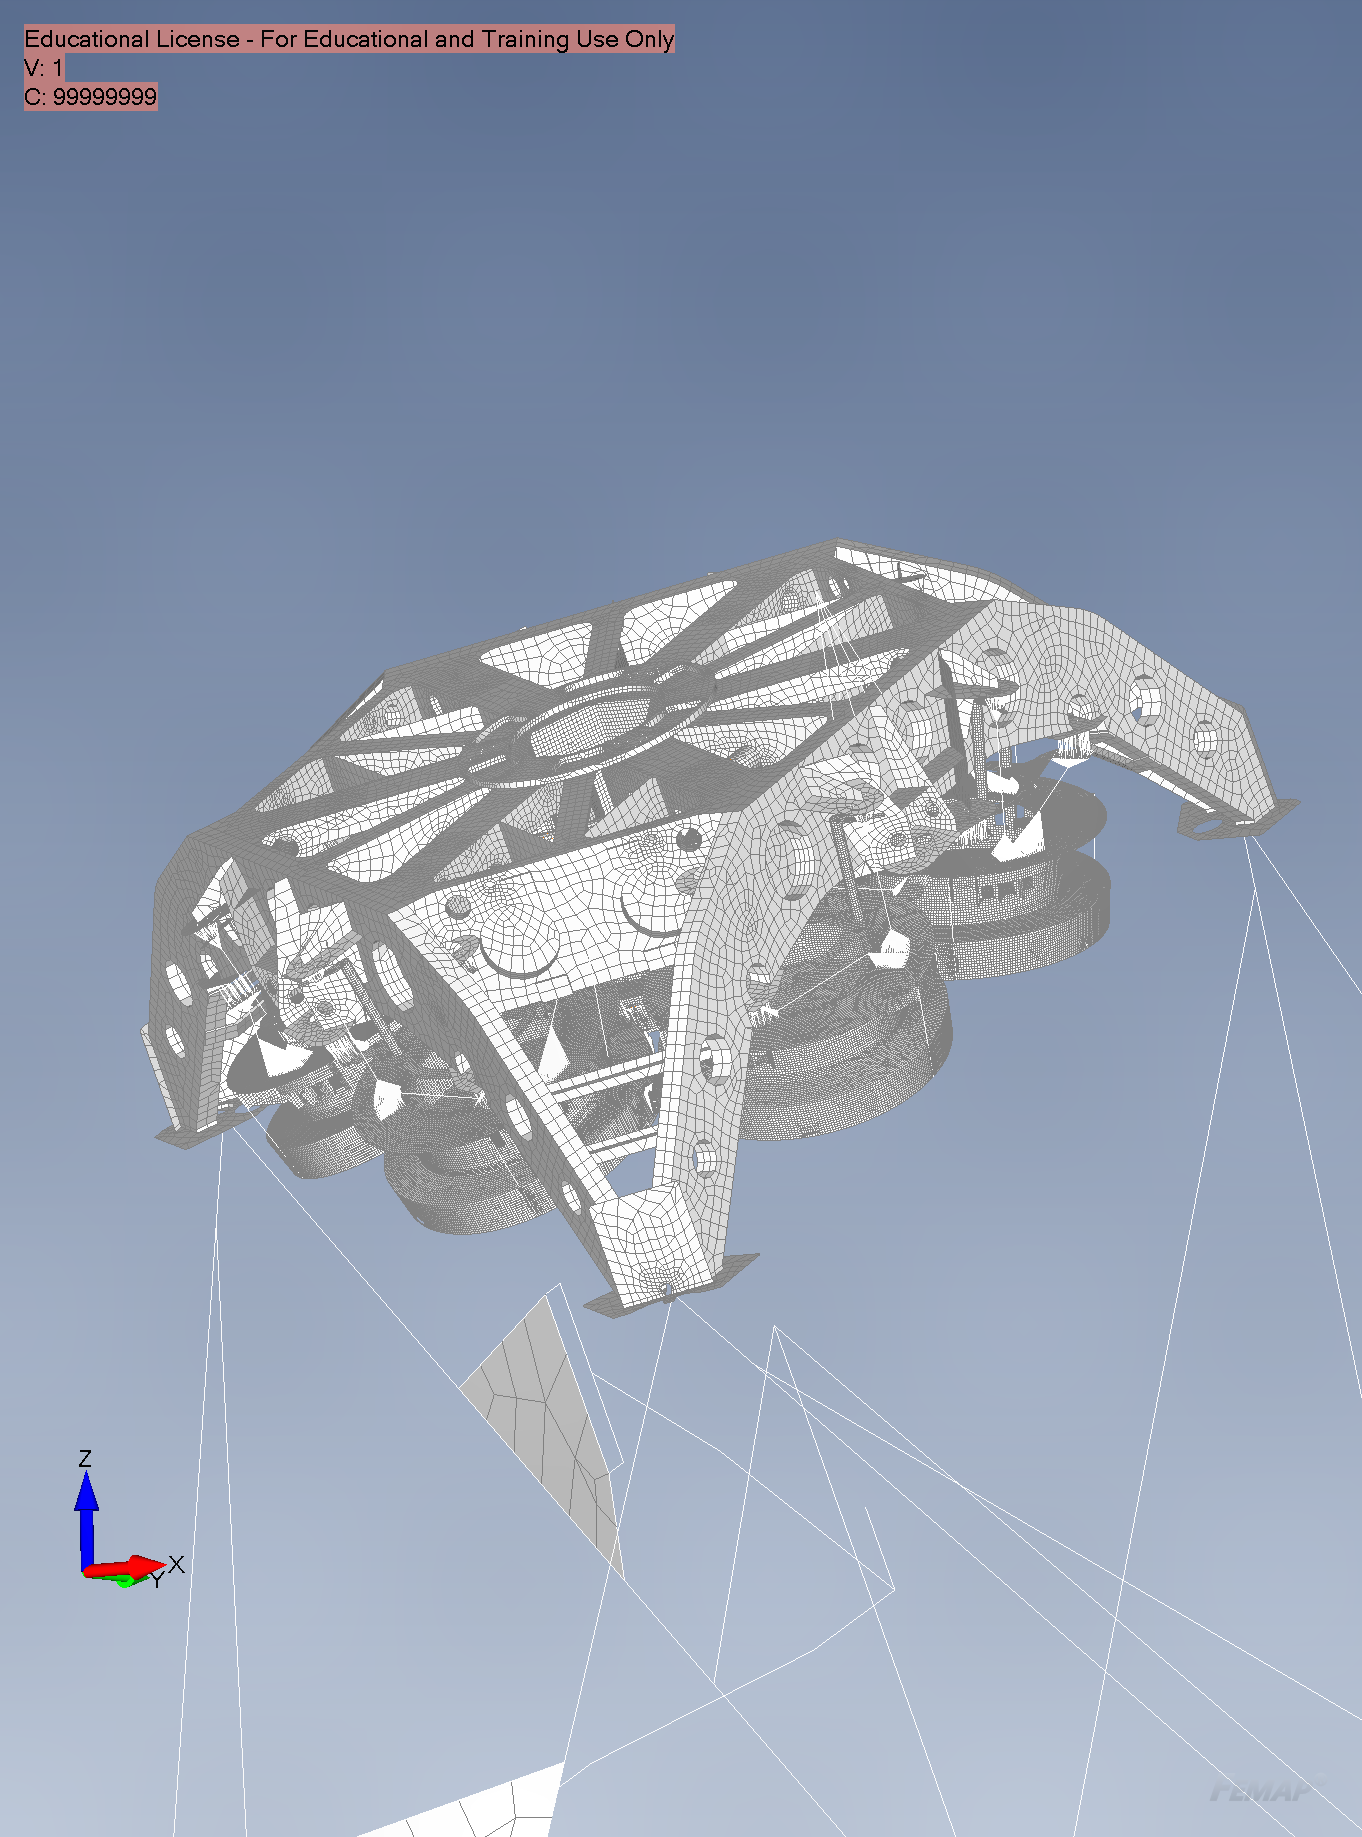
\includegraphics[width=0.6\textwidth]{FEM/topend.png}
  \caption{Top-end FEM detail.}
  \label{fig:fem-topend}
\end{figure}

\begin{figure}
  \centering
  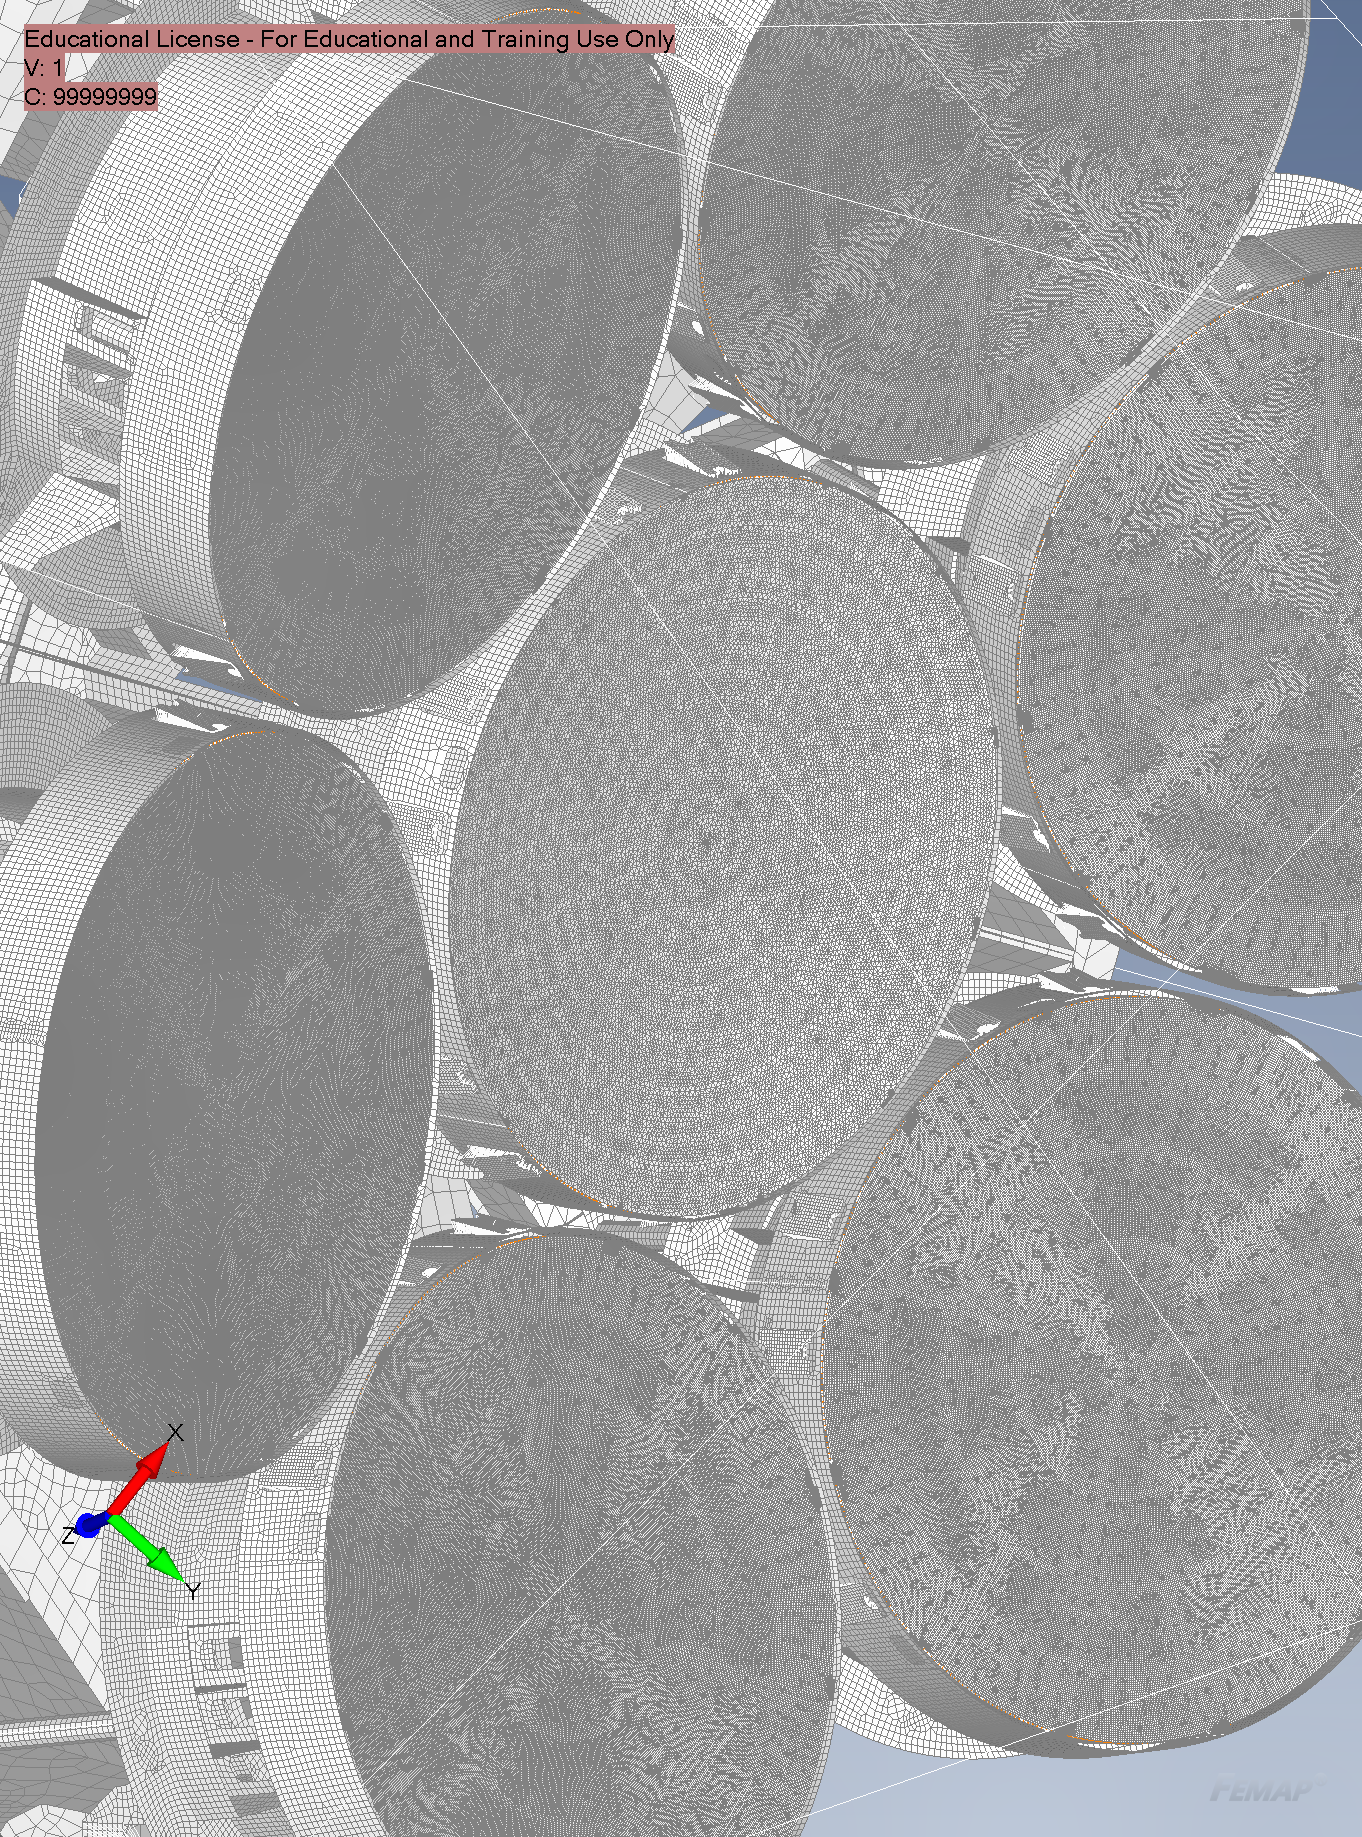
\includegraphics[width=0.6\textwidth]{FEM/facesheets.png}
  \caption{Facesheets FEM detail.}
  \label{fig:fem-facesheets}
\end{figure}

%%% Local Variables:
%%% mode: latex
%%% TeX-master: "asm-im"
%%% End:


\clearpage
\subsection{Control loops}
\label{sec:ctrlr}

%
% Control loop section
%


The control models apply temporal discrete filters to the commands sent to the actuators of the different subsystems. Figure~\ref{fig:im_control_sys} illustrates the integration of the telescope subsystems to compose the end--to--end simulator of the Natural Seeing (NS) observation mode. %
\begin{figure}[!hb]
  \centering
  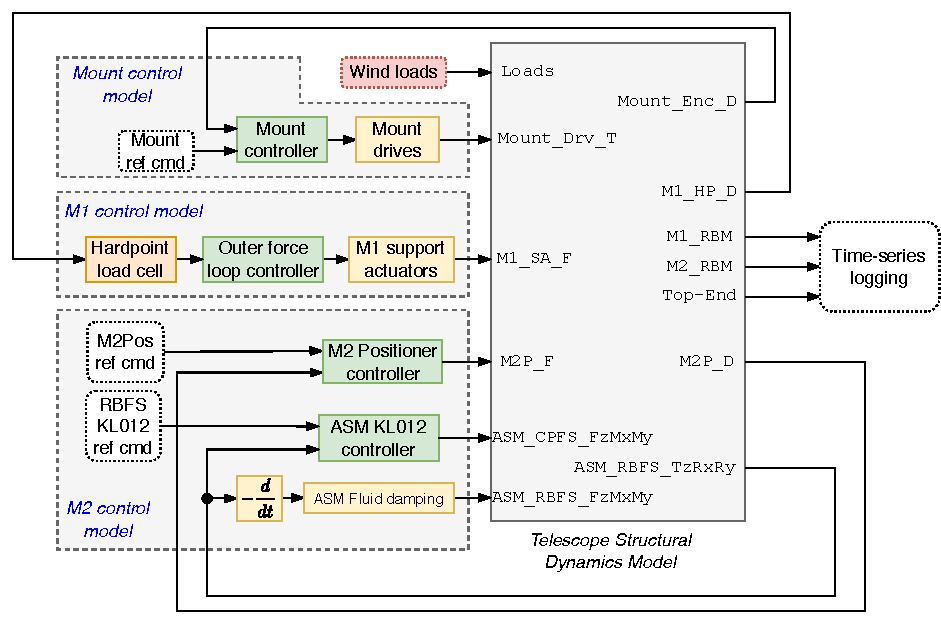
\includegraphics[width=\textwidth]{./ctrl_sec_images/pttASM_end2end_syslevel.pdf}
  \caption{Integrated model control system diagram.}
    \label{fig:im_control_sys}
  \end{figure}
In the following, we describe the main control loops incorporated into the IM framework.


\subsubsection{Mount axes control}
\label{sec:mount-ctrlr}

The mount structure shall follow a trajectory (reference command) that can be either slewing to a new science target in the sky or tracking a target. The controller ensures the mount stays on course while subject to various disturbances like gravity and wind buffeting effects. The mount controller generates compensation torque commands to the elevation, azimuth and Gregorian instrument rotator (GIR) drives to mitigate the tracking error computed based on the feedback signal of the mount axes encoders. The mount control model also considers the drive actuators by representing their dynamics and some nonlinear effects, such as quantization errors, and optionally, in a more sophisticated version, friction and parasitic torques.

Each mount axis is controlled independently using a PID compensator and notch filters to cope with structural resonant modes. A feedforward strategy is also envisioned to relieve the feedback compensator during critical acceleration/deceleration phases. 
The baseline mount controller tuning assumes structural damping of 2\%. To enable a more conservative analysis adopting a 0.5\% damping factor, GMTO~\cite{PT_IM_Jun2022} designed alternative feedback controllers for the azimuth and elevation axes. Figure~\ref{fig:mount-c-fr-plots} shows the frequency responses of the feedback controllers. 
%
\begin{figure}[!htb]
  \centering
  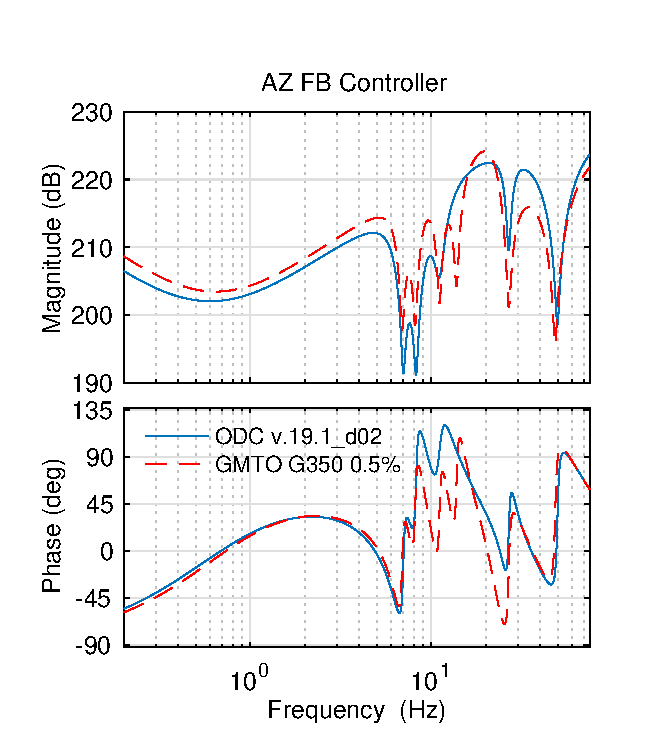
\includegraphics[width=0.32\linewidth]{./ctrl_sec_images/AZ_C_FR.eps}
    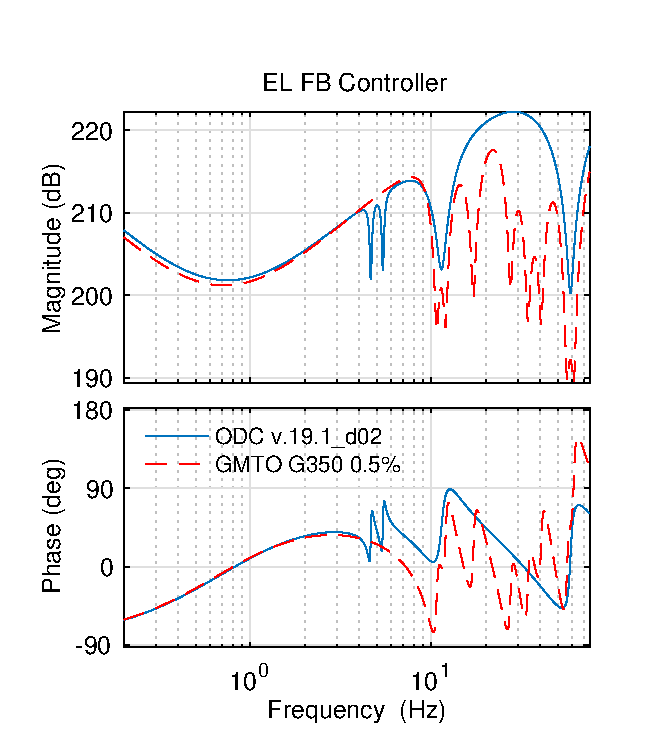
\includegraphics[width=0.32\linewidth]{./ctrl_sec_images/EL_C_FR.eps}
      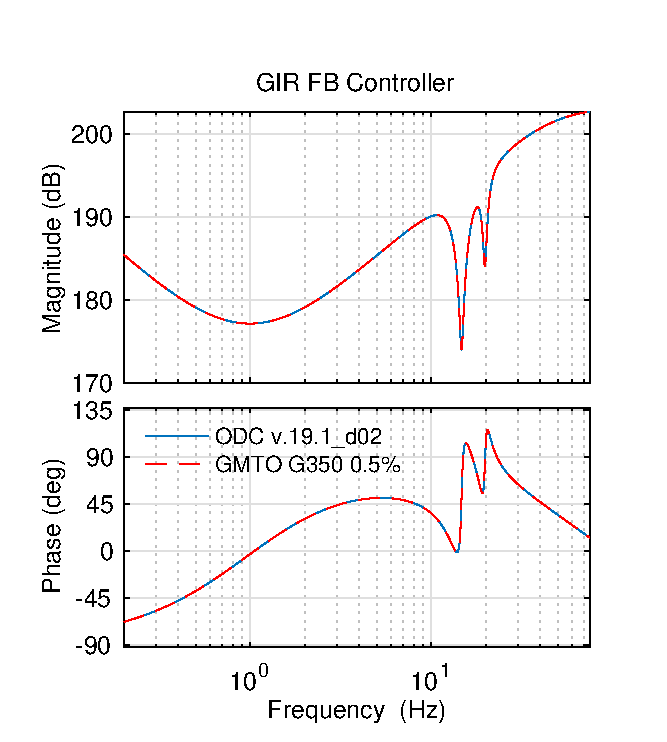
\includegraphics[width=0.32\linewidth]{./ctrl_sec_images/GIR_C_FR.eps}
  \caption{Frequency responses of the mount axes feedback controllers.}
  \label{fig:mount-c-fr-plots}
\end{figure}
%
The continuous blue line refers to the nominal ODC controller (designed under a 2\% structural damping assumption). The dashed red lines depict the frequency responses of the alternative controllers used in simulations assuming 0.5\% structural damping.

Figure~\ref{fig:mount-cl-plots} shows the closed--loop (top) and sensitivity (bottom) frequency responses of each mount axis transfer function with the elevation structure at \SI{30}{deg} zenith. The considered structural damping is 0.5\%. %
\begin{figure}[!htb]
  \centering
  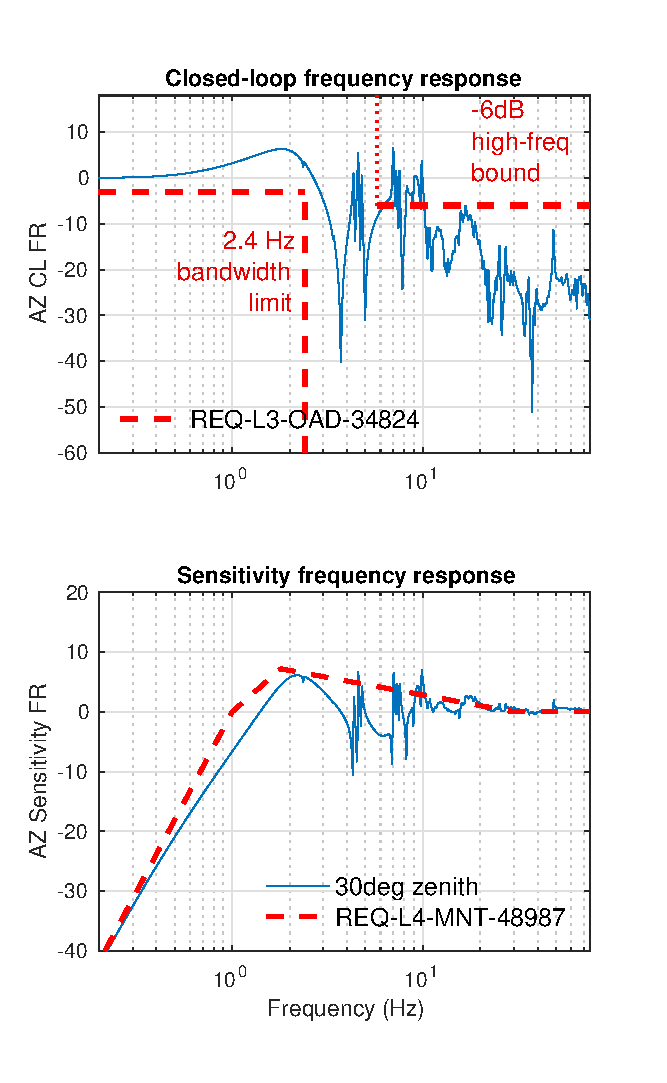
\includegraphics[width=0.32\linewidth]{./ctrl_sec_images/AZ_L3L4req_plots.eps}
    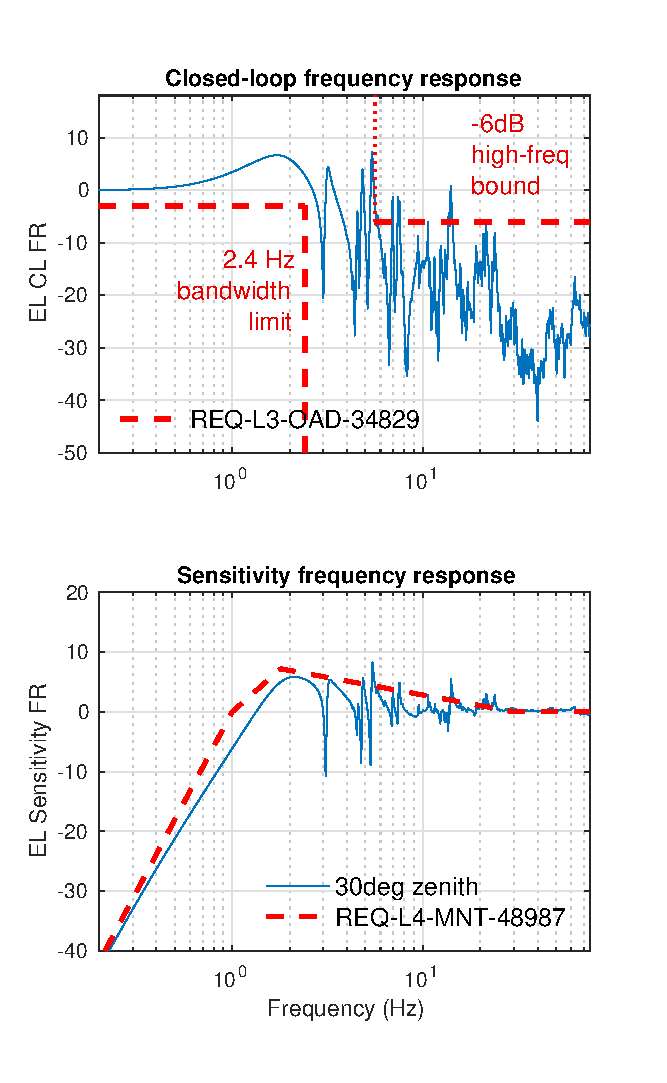
\includegraphics[width=0.32\linewidth]{./ctrl_sec_images/EL_L3L4req_plots.eps}
      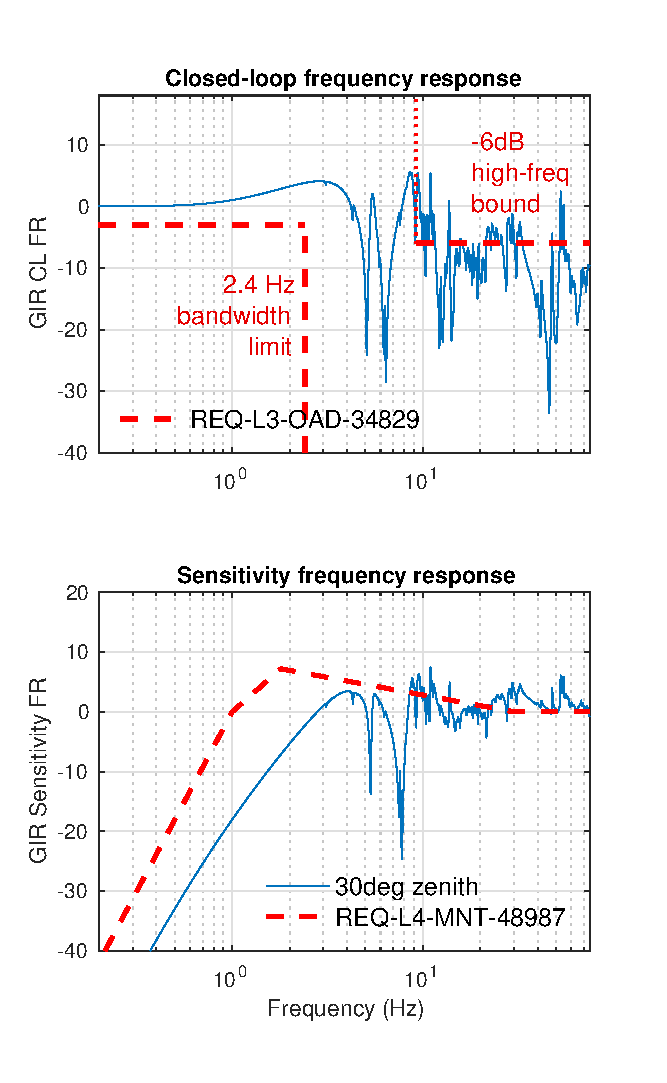
\includegraphics[width=0.32\linewidth]{./ctrl_sec_images/GIR_L3L4req_plots.eps}
  \caption{Closed--loop and sensitivity frequency responses of the mount axes transfer functions.}
  \label{fig:mount-cl-plots}
\end{figure}
%
The OAD requirements REQ--L3--OAD--34824 and REQ--L3--OAD--34829 define a \SI{2.4}{Hz} closed--loop bandwidth for the azimuth and elevation axis, respectively. The red dashed lines indicate the envelope of compliant responses. The results indicate that the OAD controller design achieves the required bandwidth. The sensitivity plots include the rejection transfer function (RTF) limits REQ--L4--MNT--48987 stated in the Mount Subsystem requirement document~\cite{MOUNT-RD}. For convenience, the envelopes in the GIR plots (on the right) assume the same requirements as those used for the azimuth and elevation axes. The obtained sensitivity transfer functions contours partially met the level--4 RTF limits. 

The mount transfer function Nichols plot (Figure~\ref{fig:mnt-nichols-plot}) slightly crosses the dashed line indicating the robustness boundary assuming a vector margin\footnote{The vector margin (VM) is the reciprocal of the maximum value of the loop sensitivity transfer function $S\left(j\omega\right)$ magnitude, i.e.$$\text{VM}=\frac{1}{\max \left|S(j\omega)\right|}.$$} (VM) of $0.5$. That indicates a limited effect on the stability margins of the feedback control system. 
\begin{figure}[!htb]
  \centering
  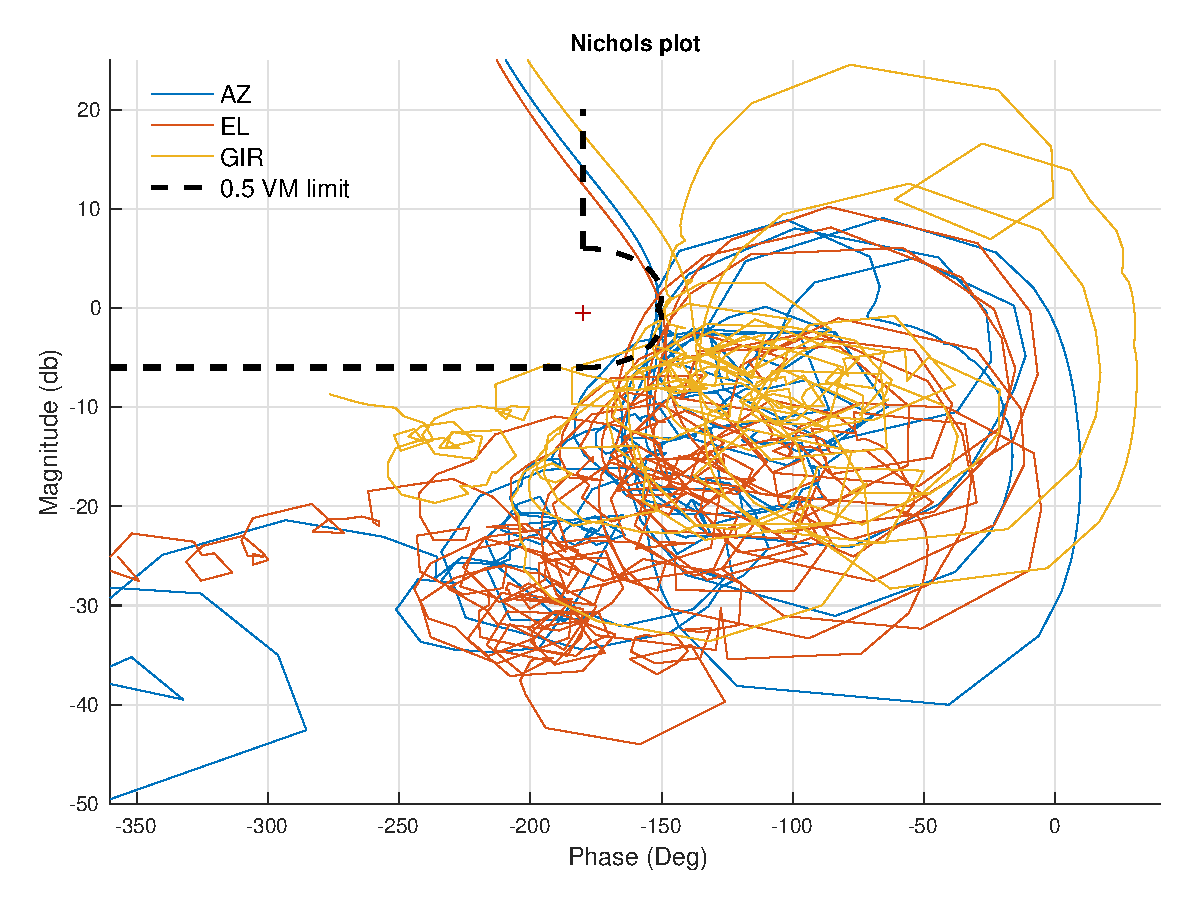
\includegraphics[width=\linewidth]{./ctrl_sec_images/all_mnt_axes_nichols.eps}
  \caption{Nichols plot of the mount axes transfer functions.}
  \label{fig:mnt-nichols-plot}
\end{figure}
Simulations also suggest that the RTF envelope violations at high--frequencies
have not led to significant performance degradation. That said, one should be
aware of that issue, particularly for a conservative 0.5\% structural damping
analysis. One can also notice that the nominal ODC GIR control design provides
\SI{4.6}{Hz} bandwidth, significantly higher than the one obtained for the other mount axes. The GIR loop disturbance rejection is also higher in the low--frequency range.



\subsubsection{M1 outer force loop}
\label{sec:m1-ctrlr}


Each primary mirror (M1) segment has six stiff actuators connected to the back of each segment, forming a hexapod. Those actuators (referred to as hardpoints, or simply HP) are also attached to the telescope mount through a cell weldment. Therefore, one defines the rigid--body position of the M1 segments by controlling the lengths of the hardpoints. In addition, the HPs have load cells mounted on the extremum of the actuator rods to measure the forces at the mirror attachment points.


The M1 force control loop is a feedback system that supports the mirror segments while minimizing the strain at the connection points with the HPs. Therefore, it relies on the measurements of the hardpoint load cells to compute commands to the M1 pneumatic support actuators (SA), which apply a force vector to the back surface of the mirrors. %These pneumatic actuators can also provide axial compensation forces to correct mirror surface figure errors through the Active Optics (AcO) control loop.


Figure~\ref{fig:m1_ofl} provides a brief representation of the M1 force loop model for each segment. %
%
\begin{figure}[!hbt]
\centering
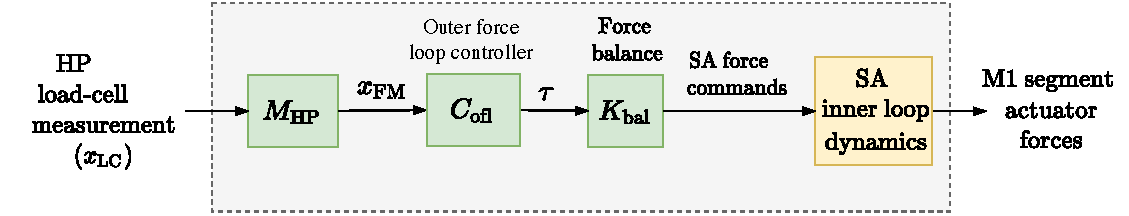
\includegraphics[width=0.7\textwidth]{./ctrl_sec_images/M1_local_control.pdf}
\caption{Primary mirror force loop control model.}
\label{fig:m1_ofl}
\end{figure}
%
 A linear transformation matrix $M_\text{hp}$ maps the HP load cell measurement signal $x_\text{LC}$ into a load vector $x_\text{FM}$ of forces and moments about the segment center of gravity (CG). The outer force loop dynamic controller $C_\text{ofl}$ computes the signal $\tau$, which compensates the load measured by the HP load cells. The controller output $\tau$ is a ``virtual'' control demand signal, as it should be distributed over the support actuators (SA) lateral, cross--lateral and axial forces. The matrix $K_\text{bal}$ accomplishes such task~\cite{GMTO.DOC.01498}. The SA compensation command drives an inner force loop, which is represented by a set of first--order linear low--pass filters with a \SI{-3}{dB} corner frequency at \SI{15}{Hz}.

 The document \cite{GMT.DOC.05153} provides a thorough description of the M1
 control system in the context of the GMT integrated model.

\subsubsection{M2 positioner}
\label{sec:m2-ctrlr}


The Observatory Requirement Document (OAD)~\cite{OAD_verF2020} stipulates through REQ--L3--OAD--35039 that the M2 positioner (M2P) shall provide a bandwidth of \SI{2}{Hz} while tracks the rigid--body motion commands.


The M2P controller computes the differential forces (\textsf{M2P\_F}), which lengthen or shorten the positioner actuators. Their lengths are the control loop feedback signals. The lengths of the M2P actuators are obtained from differential displacements of the nodes located at the extremes of the rod representing each actuator \textsf{M2P\_D}. The frequency response magnitude of the transfer functions from \textsf{M2P\_F} to \textsf{M2P\_D}, denoted hereafter as $G_\text{m2p}(s)$, are shown in Figure~\ref{fig:M2P_G}. %
%
\begin{figure}[!hbt]
    \vspace{6pt}
    \centering
    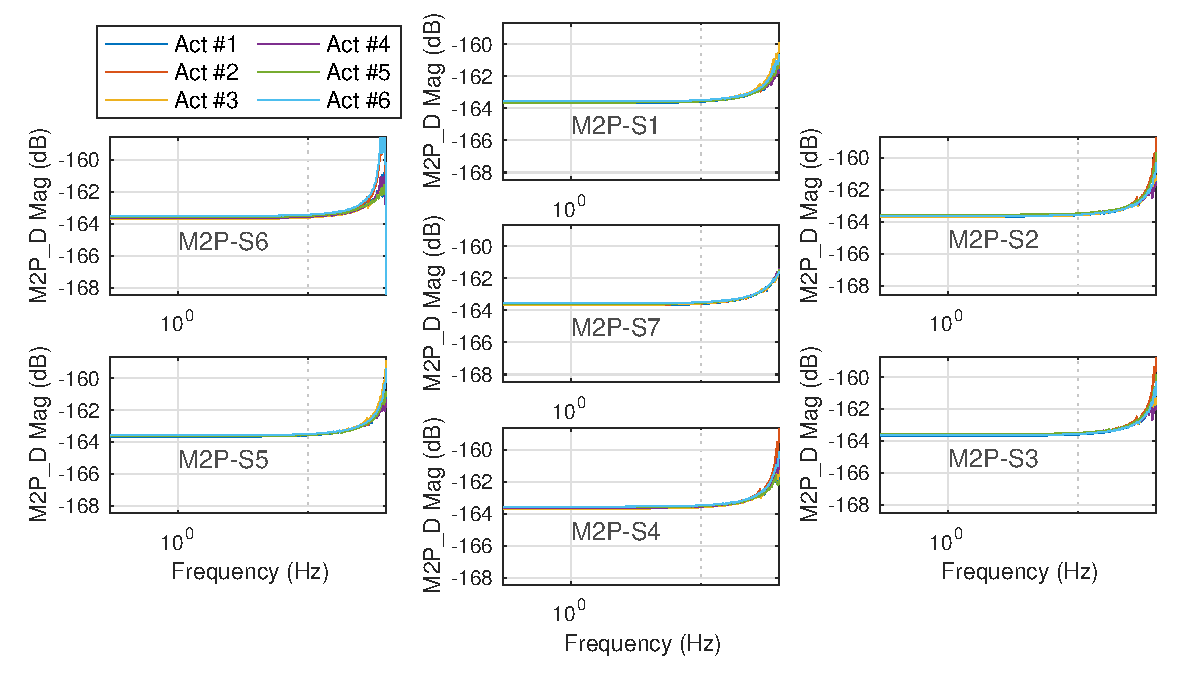
\includegraphics[width=\textwidth]{./ctrl_sec_images/M2P_G.eps}
    \caption{Frequency response magnitude of the M2 positioner actuators.}
    \label{fig:M2P_G}
\end{figure}
%
At the frequency range relevant for the specified closed--loop bandwidth, the model behaves like a static gain equal to the reciprocal of the stiffness of the M2P actuators, which is $k_\text{m2p}=\SI{158}{N/um}$. %\footnote{...}\todo{Explain difference w.r.t. FEA.}.
To provide enough gain at low frequencies and attenuate the modes above \SI{20}{Hz}, we use an M2P feedback controller with an integral term and a low--pass filter with a corner frequency at \SI{10}{Hz}, i.e.,
\begin{equation}
\label{eq:C_m2p}
C_\text{m2p}(s) = I_{42} \frac{k_{i\text{m2p}}}{s} \frac{1}{\frac{1}{\left(2\pi10\right)^2}s^2 + \frac{1}{2\pi10}s+1} ,
\end{equation}
where $I_{42}$ is a 42--dimensional identity matrix and the assumed integral gain $k_{i\text{m2p}} = 2 \pi 2 k_\text{m2p}$ leads to a unitary magnitude crossover frequency of \SI{2}{Hz}, i.e., 
\[\left|G_\text{m2p}(j\omega_0)C_\text{m2p}(j\omega_0)\right|_{\omega_0 = 2\pi2} = I_{42} .\]
%where $G_\text{m2p}(s)$ is the matrix transfer function relating the M2 differential forces \textsf{M2P\_F} and the differential displacement outputs \textsf{M2P\_D}.

The Nichols chart on the right side of Figure~\ref{fig:m2P_nichols_T} shows quite comfortable margins as the loop frequency response is distant to the dashed red line, which indicates the robustness boundary assuming a $0.5$ vector margin\footnote{The vector margin (VM) is the reciprocal of the maximum value of the loop sensitivity transfer function $S\left(j\omega\right)$ magnitude, i.e.$$\text{VM}=\frac{1}{\max \left|S(j\omega)\right|}.$$} (VM). %
%
\begin{figure}[!hbt]
    \vspace{6pt}
    \centering
    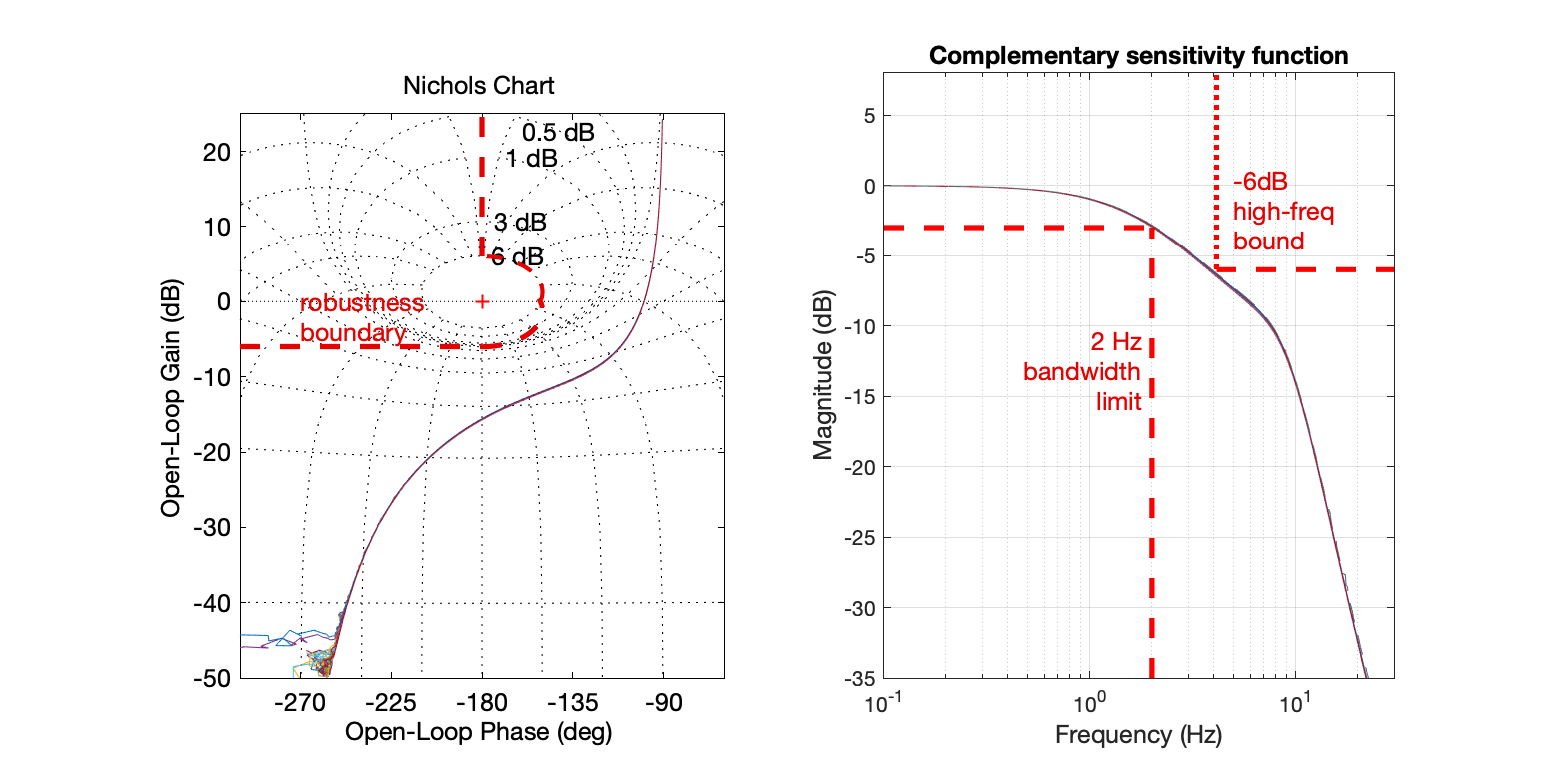
\includegraphics[width=\textwidth]{./ctrl_sec_images/m2P_nichols_T.eps}
    \caption{M2 positioner control loop characterization plots.}
    \label{fig:m2P_nichols_T}
\end{figure}
%
On the right side, one can see the closed--loop (complementary sensitivity) response of all the M2 positioner actuators. The control loop achieves the required bandwidth of \SI{2}{Hz} using the proposed feedback controller. %; see~\eqref{eq:C_m2p}.

% The matrix $K_\text{m2pT}$ maps the M2 rigid--body motion commands into reference lengths for the positioner actuators. Though $K_\text{m2pT}$ can be obtained analytically from the M2P geometry, in the context of Integrated modeling, we have computed it using the telescope structural dynamics model represented in the state--space form through the tuple $(A, B, C)$. Let $B_\textsf{M2P\_F}$ denote the partition of $B$ composed of the columns corresponding to the M2P differential force inputs \textsf{M2P\_F}. 
% Also, define $C_\textsf{M2P\_D}$ and $C_\textsf{M2\_RBM}$ as matrices constructed from the rows of $C$ corresponding to the M2P differential displacements  \textsf{M2P\_D} and the M2 rigid--body motions (\textsf{M2\_RBM}), respectively. Then
% \begin{equation*}
% K_\text{m2pT} = \bar{G}_1 \bar{G}_2^{-1},
% \end{equation*}
% where
% \begin{align*}
% \bar{G}_1 & = - C_\textsf{M2P\_D} A^{-1} B_\textsf{M2P\_F} \\
% \bar{G}_2 & = - C_\textsf{M2\_RBM} A^{-1} B_\textsf{M2P\_F}.
% \end{align*}
% %Coming from $D$, the direct feedthrough submatrices $D_1$ and $D_2$ relate the \textsf{M2P\_F} inputs and the outputs \textsf{M2P\_D} and \textsf{M2\_RBM}, respectively.



\subsubsection{ASM inner loop controller}
\label{sec:asms-ctrlr}

The ASM inner loop controller of each M2 segment has a command pre shape block, a feedback compensator, and a feedforward term. Figure~\ref{fig:asm_ctrl_diagram} shows the ASM inner loop controller block diagram. %
%
\begin{figure}[!hbt]
  \vspace{6pt}
  \centering
  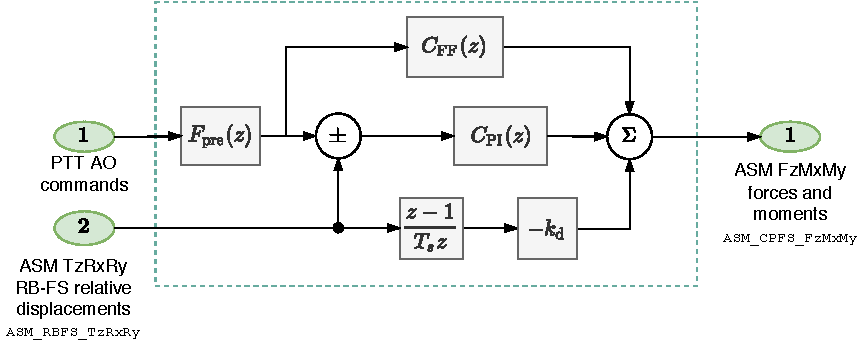
\includegraphics[width=\textwidth]{./ctrl_sec_images/pttASM_inner_loop.pdf}
  \caption{ASM inner loop controller diagram.}
  \label{fig:asm_ctrl_diagram}
\end{figure}
%
The PI+D controller uses the differential $T_z$ (translation along $\overrightarrow{z}$), $R_x$ and $R_y$ (rotations about the $\overrightarrow{x}$ and $\overrightarrow{y}$ axes of the M2 local coordinate system, respectively) displacements between the reference body (RB) and the face sheet (FS) of each segment as feedback signals. %
The $21$--dimensional $C_\text{PI}$ transfer function matrix is strictly diagonal, whose nonzero terms are discrete--time versions of
\begin{equation*}
%\label{eq:pi_CT}
C_\text{PI}(s) = \left(k_p + \frac{k_i}{s} \right).
\end{equation*}
An electronic damping correction (derivative action) proportional to $k_d$ also composes the feedback controller. Let $T_s$ the sampling period; in the current version, the forward approximation $$\frac{d}{dt} \approx \frac{1}{T_s}\frac{z-1}{z}$$ provides the numerical differentiation of the relative displacements between the ASM reference bodies and face sheets. %
%
As reported in Table~\ref{tab:ASM_inner_ctrl_par}, the controller model gains (namely, $k_p$, $k_i$, and $k_d$) assume different values for piston and tip--tilt modes.
\begin{table}[!htb]
  \centering
  \caption{ASM inner loop controller model parameters.}
  \label{tab:ASM_inner_ctrl_par}
  \begin{tabular}{l|ccc}
  %\hline
  & $k_p$ & $k_i$ & $k_d$\\
  \hline
  Piston & $47.25 \times 10^6$~\SI{}{N/m} & $3.375 \times 10^8$~\SI{}{N/(m s)} & $1.6538 \times 10^4$~\SI{}{Ns/m}\\
  %\hline
  Tip--tilt & $3.3034 \times 10^6$~\SI{}{N/m} & $2.3596 \times 10^7$~\SI{}{N/m} & $1.1562 \times 10^3$~\SI{}{Ns/m}\\
  %\hline
  \end{tabular}
  \end{table}

The command pre-shape block aims at smoothing the 21--dimensional optical controller command vector $r_\text{AO}$ using a $4^{th}$--order Bessel filter with \SI{2200}{Hz} corner frequency. 
The feedforward (FF) control has a static and dynamic contribution. The purpose of the static contribution is to provide (in advance) the static forces required to apply a particular command, statically decoupling all the commanded degrees of freedom. The dynamic FF term aims at pre-compensating (in open-loop) the system dynamics during the command transients. 
As can be seen in Figure 7, both the pre-shape filter and the feedforward term are not excited when the PTT commands are set to zero, which is the case for the simulations performed to generate wind-induced motion to AdOptica. The ASMS Phasing System Analysis Report~\cite[Section~4.1.3]{ADP_PhasingRep2021} describes in more detail the pre-shape filter and feedforward action of the inner ASM controller.

The ASM controller is realized at a uniform sampling rate of \SI{8}{KHz} ($Ts = 1.25 \times 10^{-4}$~\SI{}{s}). One obtains the pre--shape filter transfer function $F_\text{pre}(z)$ and the PI controller $C_\text{PI}(z)$ applying the trapezoidal (Tustin) discretization method to the respective continuous--time representations. %


\subsubsection*{Dynamic fluid damping}

Assuming a frequency range of interest of a few hundredths of Hz, the fluid dynamic forces can be simplified to pure linear fluid dynamic damping. From the modeling point of view, in this version, the fluid dynamic damping is represented by an ideal feedback loop introducing a pure damping contribution proportional to the motion velocity between the RBs and the mirrors FS. 

Let, $y_\text{RbFs} \in \mathbb{R}^{21}$ the relative displacement projected onto the piston and tip--tilt modes. The fluid damping vector $u_\text{fd}$ applied as forces (along $\overrightarrow{z}$) and moments (about $\overrightarrow{x}$ and $\overrightarrow{y}$) to the ASM reference body and with opposite sign to the face sheets reads as
\[
u_\text{fd} = -k_\text{fd} \left(\frac{1}{T_s}\frac{z-1}{z}\right) y_\text{RbFs}.
\]
where $k_\text{fd}$ is $6.1425\times 10^{3}$~\SI{}{Ns/m} and $4.2945\times 10^{2}$~\SI{}{Ns/m} for piston and tip--tilt modes, respectively. 
%




\subsection{Wind loads}
\label{sec:wind-loads}

The wind loads applied to FEM of the telescope have been computing with
Computational Fluid Dynamics (CFD) simulations.
The CFD model\cite{GMT.DOC.05211} of the telescope and enclosure is based on CAD drawings released
for the PDR of the GMT mount and the GMT enclosure.
A database of dome seeing, wind loads and heat transfer coefficients from 60 CFD
simulations covering a range of wind speed and orientation,
telescope pointing and enclosure configurations have been
built\cite{GMT.DOC.05214}.

Using the CFD wind loads on the telescope FEM,
the time series of rigid body motions of M1 and M2 segments and of the
truss--to--top-end interface have been computed for 15 CFD cases, as listed in
Table~\ref{tab:cfd-cases}.
The mapping and transformations of the CFD wind loads to FEM wind loads is
described in \cite{GMT.DOC.05506}.

\begin{table}
  \centering
  \begin{tabular}{c}
    -
  \end{tabular}
  \begin{tabular}{ccccc}\toprule
    Zenith & Azimuth & Vents  & Wind screen & Wind speed \\
    deg & deg & - & - & m/s \\\midrule
    30     & 0       & open & stowed & 2 \\ 
    30     & 0       & open & stowed & 7 \\ 
    30     & 0       & closed & deployed & 12 \\ 
    30     & 45       & open & stowed & 2 \\ 
    30     & 45       & open & stowed & 7 \\ 
    30     & 45       & closed & deployed & 12 \\ 
    30     & 45       & closed & deployed & 17 \\ 
    30     & 90       & open & stowed & 2 \\ 
    30     & 90       & open & stowed & 7 \\ 
    30     & 90       & closed & deployed & 12 \\ 
    30     & 135       & open & stowed & 7 \\ 
    30     & 135       & closed & deployed & 12 \\ 
    30     & 180       & open & stowed & 7 \\ 
    30     & 180       & closed & deployed & 12 \\ 
    60     & 45       & open & stowed & 7 \\ \bottomrule
  \end{tabular}
  \label{tab:cfd-cases}
  \caption{List of CFD cases used to compute the wind motions time series.}
\end{table}




%%% Local Variables:
%%% mode: latex
%%% TeX-master: "asm-im"
%%% End:


\appendix

\section{Validation and tests}
\label{sec:tests}

\subsection{FEM}
\label{sec:fem-tests}

\subsection{Controllers}
\label{sec:ctrlr-tests}




\printbibliography


\end{document}
